\section{Results}
We ran three data trials: “canny, dotted, stripe”, “shear, canny, spatter”, and “stripe, motion, scale”. For each trial, we applied the KNN and the RF classifiers from the scikit-learn library. The KNN was executed from k=3 to k=10000, and the RF was fit with estimators of 3, 10, and 30.

The KNN performance was heavily sensitive to the data selected, whereas the RF was not so sensitive. In general, the KNN had poor performance, while the RF did a very good job detecting the anomalies.

\begin{figure}[htbp]
    \centerline{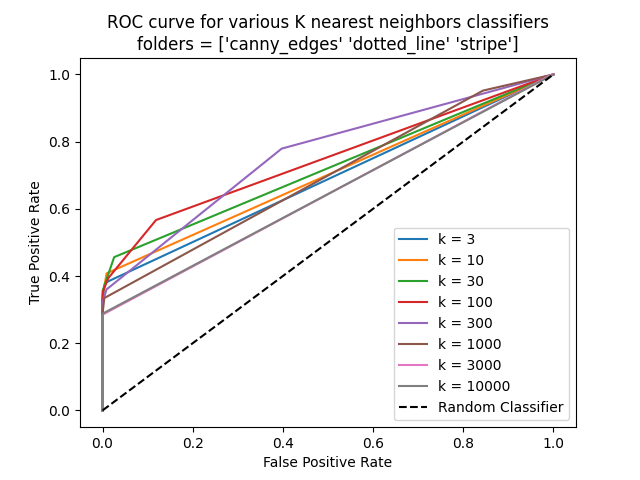
\includegraphics[width=0.5\textwidth]{resources/roc_curve_knn_canny_edges_dotted_line_stripe.png}}    
    \caption{ROC Curve for KNN: with canny edges, dotted lines and striped}\label{fig9}
\end{figure}

\begin{figure}[htbp]
    \centerline{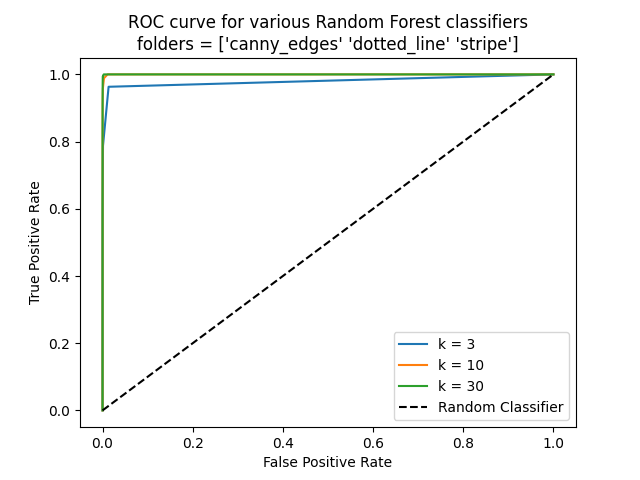
\includegraphics[width=0.5\textwidth]{resources/roc_curve_rf_canny_edges_dotted_line_stripe.png}}    
    \caption{ROC Curve for RF: with canny edges, dotted lines and striped}\label{fig10}
\end{figure}

\begin{figure}[htbp]
    \centerline{\includegraphics[width=0.5\textwidth]{resources/precision_recall_knn_canny_edges_dotted_line_stripe.png}}    
    \caption{PR Curve for KNN: with canny edges, dotted lines and striped}\label{fig11}
\end{figure}

\begin{figure}[htbp]
    \centerline{\includegraphics[width=0.5\textwidth]{resources/precision_recall_rf_canny_edges_dotted_line_stripe.png}}    
    \caption{PR Curve for RF: with canny edges, dotted lines and striped}\label{fig12}
\end{figure}

\begin{figure}[htbp]
    \centerline{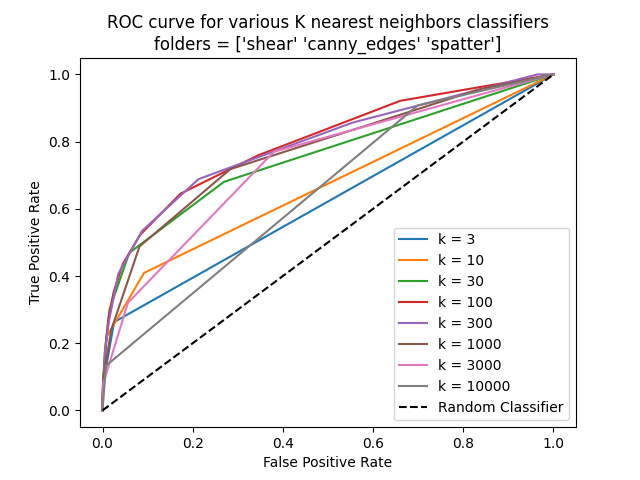
\includegraphics[width=0.5\textwidth]{resources/roc_curve_knn_shear_canny_edges_spatter.png}}    
    \caption{ROC Curve for KNN: with shear, canny edges, and spatter}\label{fig13}
\end{figure}

\begin{figure}[htbp]
    \centerline{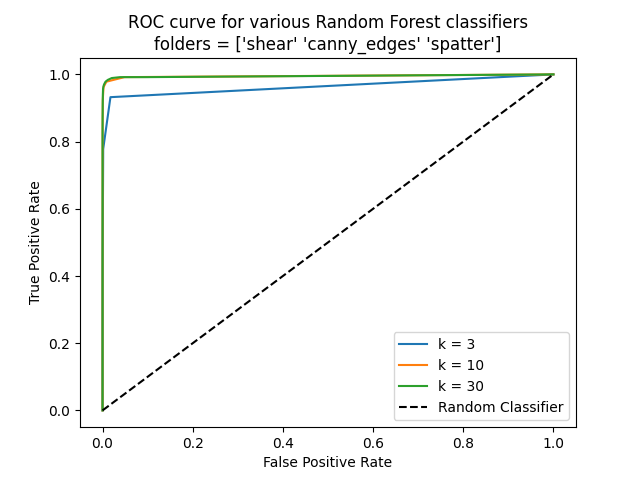
\includegraphics[width=0.5\textwidth]{resources/roc_curve_rf_shear_canny_edges_spatter.png}}    
    \caption{ROC Curve for RF: with shear, canny edges, and spatter}\label{fig14}
\end{figure}

\begin{figure}[htbp]
    \centerline{\includegraphics[width=0.5\textwidth]{resources/precision_recall_knn_shear_canny_edges_spatter.png}}    
    \caption{PR Curve for KNN: with shear, canny edges, and spatter}\label{fig15}
\end{figure}

\begin{figure}[htbp]
    \centerline{\includegraphics[width=0.5\textwidth]{resources/precision_recall_rf_shear_canny_edges_spatter.png}}    
    \caption{PR Curve for RF: with shear, canny edges, and spatter}\label{fig16}
\end{figure}

\begin{figure}[htbp]
    \centerline{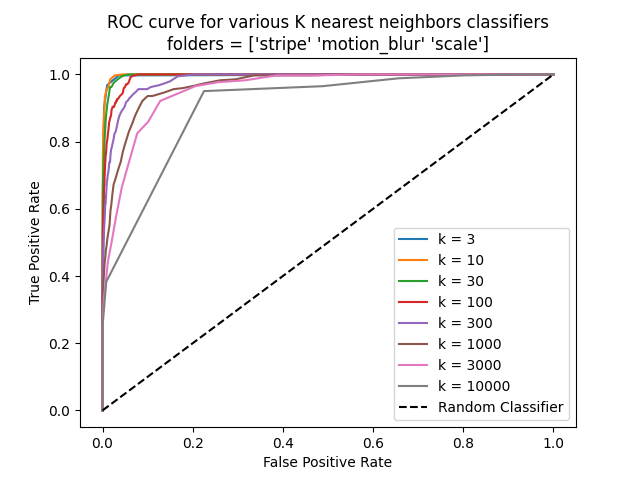
\includegraphics[width=0.5\textwidth]{resources/roc_curve_knn_stripe_motion_blur_scale.png}}    
    \caption{ROC Curve for KNN: with striped, motion blur, and scale}\label{fig17}
\end{figure}

\begin{figure}[htbp]
    \centerline{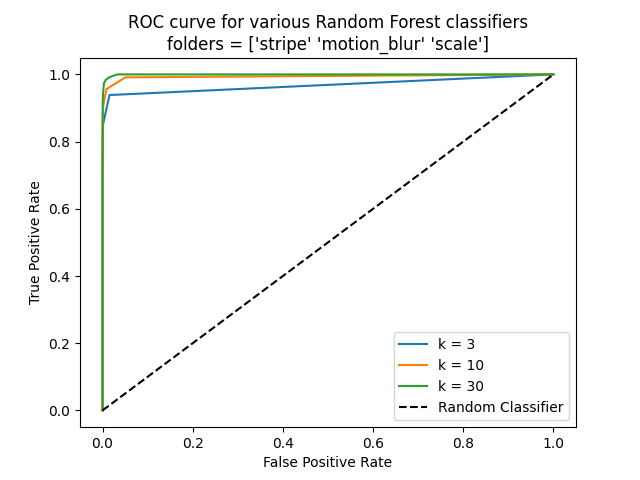
\includegraphics[width=0.5\textwidth]{resources/roc_curve_rf_stripe_motion_blur_scale.png}}    
    \caption{ROC Curve for RF: with striped, motion blur, and scale}\label{fig18}
\end{figure}

\begin{figure}[htbp]
    \centerline{\includegraphics[width=0.5\textwidth]{resources/precision_recall_knn_stripe_motion_blur_scale.png}}    
    \caption{PR Curve for KNN: with striped, motion blur, and scale}\label{fig19}
\end{figure}

\begin{figure}[htbp]
    \centerline{\includegraphics[width=0.5\textwidth]{resources/precision_recall_rf_stripe_motion_blur_scale.png}}    
    \caption{PR Curve for RF: with striped, motion blur, and scale}\label{fig20}
\end{figure}

\section{Conclusion}

This assignment provided valuable experience to use various probability density-based anomaly detectors and evaluating their performance using ROC and PR curves.
Despite the challenges posed by the MNIST-C dataset, the RF classifier performed well in detecting anomalies, while the KNN classifier struggled to achieve similar results. 
The RF classifier was less sensitive to the data selected, which made it a more robust choice for anomaly detection in this context.   


\section{Appendix: Code Summary}





The provided Python code, $csc730\_assignment\_6\_KJ.ipynb$ ,  is a comprehensive Jupyter notebook for processing and analyzing the MNIST dataset, a large database of handwritten digits. The code also handles corrupted versions of the MNIST dataset, which are used to simulate anomalies in the data. 
The analysis involves the use of machine learning algorithms, specifically the k-nearest neighbors classifier (KNN) and the random forest classifier (RF).
The code begins by setting up several variables related to the MNIST and corrupted MNIST datasets (MNIST-C), including paths to the data, flags indicating whether the data has been downloaded or files have been generated, and parameters for the corruption process. 
It also initializes empty lists to store the results of the machine learning models.\par

The $process\_data$ function is defined to handle the downloading and preprocessing of the MNIST data. 
If the data has not been downloaded, it fetches the MNIST dataset from OpenML. 
If the MNIST files have not been generated, it loads the data, converts it to numpy arrays, reshapes the images, and saves the processed data to disk. 
It also splits the data into training and testing sets.\par

If the $generate\_corrupted\_data$ flag is set, the code generates corrupted versions of the MNIST data.
It randomly selects a number (default=3) of corruption types, applies them to a subset of the data, and concatenates the corrupted data with the original MNIST data. 
The labels for the corrupted data are also generated and saved. These generated labels follow this function.\par
$L_a(x) = 
\begin{cases} 
1 & \text{if } x.source = MNIST-C \text{ (anomalous)} \\
0 & \text{if } x.source = MNIST \text{ (nominal)}
\end{cases}$ \par

The code then loads the MNIST and corrupted MNIST data and labels from disk. 
It reshapes the images into a 2D format suitable for the machine learning models and splits the data into training and testing sets.\par

For each specified number of neighbors in $knnc\_test\_scenarios$, the code fits a KNN model to the training data, makes predictions on the testing data, and stores the predicted labels and probabilities. 
It does a similar process for the specified number of estimators in $rf\_test\_scenarios$ using a RF model.\par

The $generate\_roc\_curve$ function is defined to generate a ROC curve for the KNN and RF models. 
For each model and each threshold, it calculates the true positive rate (TPR) and false positive rate (FPR), and plots these rates to create the ROC curve.\par

The $generate\_precision\_recall\_curve$ function is defined to generate a PR curve for the KNN and RF models. 
For each model and each threshold, it calculates the precision and recall, and plots these values to create the PR curve.\par

Finally, the code calls the $generate\_roc\_curve$ and $generate\_precision\_recall\_curve$ functions to generate and save the ROC and PR curves for the KNN and RF models. The curves are saved as PNG images and displayed in the notebook.\par






